\section{Introduccion a redes neuronales de funcioness Base Radial}

La arquitectura de las redes RBF está formada por una capa de entrada, una capa oculta y una capa de salida, está última será la suma ponderada de las salidas de la RBFs en caso de Regresión y será de tipo Softmax en caso de Clasificación. Las redes neuronales de funciones de base Radial (RBF) se basan en una aproximación local.
\begin{itemize}
\item Las neuronas de capa oculta son funciones de base radial: Son funciones locales. Dividen el espacio mediante hiperesferas, una por cada neurona de capa oculta, en las cuales se define un centro y un radio.
\item Al contrario de las redes de tipo perceptrón multicapa, donde las neuronas son de capa oculta son funciones de tipo sigmoide: Estas son funciones de proyección.
\end{itemize}
A continuación en la Figura \ref{fig:diferencias_funciones} se puede comprobar las diferencias.
\begin{figure}[ht]
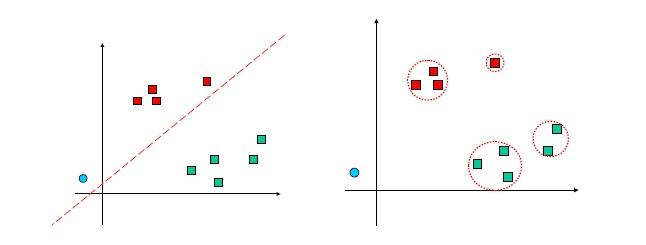
\includegraphics[scale=1]{img/img1.jpg}
\caption{Izq: Función proyección, Der: Función local}
\label{fig:diferencias_funciones}
\end{figure}

Las funciones RBF dependen de la distancia que hay entre la entrada y un centro, cada RBF guarda un centro como referencia, y cada vez que se le presenta un patrón nuevo, se calcula la distancia a dicho centro. Para calcular la distancia de un patrón entre centros se usará los radios.
\begin{itemize}
	\item Si la distancia es pequeña, la RBF se activa (su salida es 1).
	\item Si la distancia es grande, la RBF no se activa (su salida es 0).
	\item Si el radio es pequeño, la activación solo se producirá cuando el patrón esté muy cerca del centro.
	\item Si el radio es grande, la activación se producirá a más distancia.
\end{itemize}

¿Como ajustamos los parámetros?, aunque las funciones RBF son derivables, son bastantes complejas y tienen un coste computacional alto, por lo tanto emplearemos un entrenamiento Híbrido: parte no supervisada (clustering) y parte supervisada (regresión logística o inversión de una matriz).

